\documentclass[11pt,letterpaper]{book}

%-----------------------PAQUTES---------------------------%
\usepackage{graphicx}
\usepackage[spanish]{babel}
\usepackage{float}

\usepackage{courier} %% Sets font for listing as Courier.
\usepackage{listings, xcolor}
\lstset{
tabsize = 4, %% set tab space width
showstringspaces = false, %% prevent space marking in strings, string is defined as the text that is generally printed directly to the console
numbers = left, %% display line numbers on the left
commentstyle = \color{green}, %% set comment color
keywordstyle = \color{blue}, %% set keyword color
stringstyle = \color{red}, %% set string color
rulecolor = \color{black}, %% set frame color to avoid being affected by text color
basicstyle = \small \ttfamily , %% set listing font and size
breaklines = true, %% enable line breaking
numberstyle = \tiny,
}
%\usepackage{listings}
%\usepackage{color}
%------------------------MACROS---------------------------%
%\definecolor{mygreen}{rgb}{0,0.6,0}
\definecolor{mygray}{rgb}{0.5,0.5,0.5}
\definecolor{mymauve}{rgb}{0.58,0,0.82}

\lstset{ 
  backgroundcolor=\color{white},   % choose the background color; you must add \usepackage{color} or \usepackage{xcolor}; should come as last argument
  basicstyle=\footnotesize,        % the size of the fonts that are used for the code
  breakatwhitespace=false,         % sets if automatic breaks should only happen at whitespace
  breaklines=true,                 % sets automatic line breaking
  captionpos=b,                    % sets the caption-position to bottom
  commentstyle=\color{mygreen},    % comment style
  deletekeywords={...},            % if you want to delete keywords from the given language
  escapeinside={\%*}{*)},          % if you want to add LaTeX within your code
  extendedchars=true,              % lets you use non-ASCII characters; for 8-bits encodings only, does not work with UTF-8
  firstnumber=1000,                % start line enumeration with line 1000
  frame=single,	                   % adds a frame around the code
  keepspaces=true,                 % keeps spaces in text, useful for keeping indentation of code (possibly needs columns=flexible)
  keywordstyle=\color{blue},       % keyword style
  language=Octave,                 % the language of the code
  morekeywords={*,...},            % if you want to add more keywords to the set
  numbers=left,                    % where to put the line-numbers; possible values are (none, left, right)
  numbersep=5pt,                   % how far the line-numbers are from the code
  numberstyle=\tiny\color{mygray}, % the style that is used for the line-numbers
  rulecolor=\color{black},         % if not set, the frame-color may be changed on line-breaks within not-black text (e.g. comments (green here))
  showspaces=false,                % show spaces everywhere adding particular underscores; it overrides 'showstringspaces'
  showstringspaces=false,          % underline spaces within strings only
  showtabs=false,                  % show tabs within strings adding particular underscores
  stepnumber=2,                    % the step between two line-numbers. If it's 1, each line will be numbered
  stringstyle=\color{mymauve},     % string literal style
  tabsize=2,	                   % sets default tabsize to 2 spaces
  title=\lstname                   % show the filename of files included with \lstinputlisting; also try caption instead of title
}
%-----------------------PORTADA---------------------------%
\title{Proyecto Final}
\author{Estefanía García González, Sebastián Mora Sabogal}
\begin{document}
\maketitle
\tableofcontents
\listoffigures

\part{PROYECTO}
\chapter{Caso de Estudio}
\section{Introducción}
Desde que el ser humano cuenta con raciocinio , ha buscado organizarse, desarrollar metodologías y nuevas tecnologías que faciliten su diario vivir. Ha habido un recorrido histórico en el cual las necesidades humanas de optimización de tiempo y recursos han ido en aumento, así mismo las soluciones a éstas. 
En los últimos años se ha podido apreciar una constante migración al uso de tecnologías de la información que permiten realizar a cabo tareas en todos los ámbitos de forma óptima. Uno de los actores que más se han visto inmersos en la revolución digital son los estudiantes, pero en su contexto universitario, hace falta desarrollar estrategias que le permitan mejorar la gestión de tiempo de sus actividades académicas; por lo cual se buscará una solución tecnológica que se adapte a las necesidades de los universitarios.
\section{Objetivo General}
Desarrollar un software que gestione actividades y tiempos de las asignaciones académicas a estudiantes universitarios, utilizando los modelos y metodologías de ingeniería de software para mejorar la productividad del universitario.

\section{Objetivos Específicos}
\begin{enumerate}
	\item Analizar el problema teniendo en cuenta la observación de las necesidades del estudiante, para así enfocarse en estos elementos primordiales a la hora de desarrollar el software.
	\item Presentar una solución a nivel de software a partir del previo análisis del problema para finalmente implementarlo. 
	
\end{enumerate}
\section{Descripción del problema}
La vida universitaria y académica suele ser difícil de manejar debido a la cantidad de trabajos que se deben entregar diariamente, a la prioridad que cada una es para el usuario y a la gestión de tiempo para poder realizarlos. Tareas, trabajos, talleres y grandes proyectos son algunas de las actividades que un estudiante realiza durante su semestre; además de que cada uno tiene complejidad y tiempo de realización diferentes estimados por el estudiante.
Una solución factible es la utilización de un software gestor de tareas orientado a la organización y  optimización de actividades académicas.

\section{Alcance}
Este software tendrá la capacidad de gestionar los horarios de los estudiantes, añadir recordatorios de trabajos próximos a presentar y ofrecer el servicio de organizar en horarios la realización de las tareas pendientes. Esto se llevará a cabo de acuerdo a la complejidad de la actividad a realizar, en la cual se tomará en cuenta el nivel de dificultad, si se puede desarrollar en diferentes etapas y la fecha de entrega. 

El estudiante estará en la capacidad de añadir actividades, determinar la complejidad de éstas y asignarles un horario de realización que puede ser repartido en varios bloques cuando la tarea requiere de mucho tiempo. Adicionalmente, las actividades podrán personalizarse añadiendoles objetivos a cumplir o subactividades.


\chapter{Metodología}
\section{Introducción}
contenido ...
\newpage

\section{Proceso de Software}
Parte importante de un proyecto de software es definir el, o los ciclos de vida que se manejarán dentro del proyecto, ya que estos determinarán estrategias para planificar,desarrollar y mantener el software. Por esta razón, se definirá el modelo de procesos a utilizar, tomando en cuenta los siguientes criterios:
\begin{itemize}
	\item Es necesaria una metodología que sea pertinente para un proyecto de software pequeño con pocos desarrolladores.
	\item Se considera importante la verificación en cada fase del ciclo de vida, ya que permite sentar buenas bases dentro del proyecto y reducir el riesgo.
	\item Además de la verificación, es necesaria una retroalimentación constante, ya que es posible ver con mayor claridad las falencias y carencias del proyecto.
	\item Como último criterio fundamental, se contempla la necesidad de desarrollar algunas partes de software de forma rápida, ya que esto facilitaría la retroalimentación del sistema.
\end{itemize}
Para cumplir con las pautas anteriormente mencionadas, los ciclos de vida que se elegirán son prototipo y V. Cada uno de estos modelos obedece solo a algunas de las especificaciones, pero juntos se complementan de la siguiente manera:
\begin{itemize}
	\item El modelo V es perfecto para equipos de trabajo pequeños, ya que es sencillo, de fácil aprendizaje, robusto e incluye pruebas en cada fase, lo que facilita el trabajo cuando hay pocas personas. 
	\item Gracias a los dos ciclos de vida, es posible hacer una verificación y retroalimentación de forma efectiva, ya que con el modelo en V se hacen pruebas en cada fase y con el prototipo es posible obtener resultados a corto plazo que se pueden ir revisando y evaluando.
	\item El modelo de prototipo brinda la posibilidad de construir partes del proyecto de forma prematura, por lo que es posible realizar pruebas y verificar qué cosas es necesario cambiar o añadir.
\end{itemize}
\begin{figure}
	\centering
	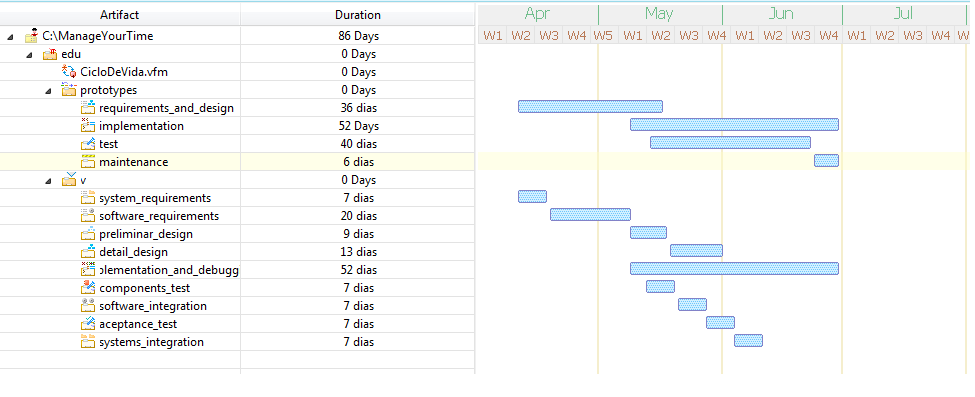
\includegraphics[width=0.7\linewidth]{proyecto/metodologia/imgs/Gantt}
	\caption{}
	\label{fig:gantt}
\end{figure}
\subsection{Metodología de implementación}
Los criterios que se establecieron al momento de justificar la elección los procesos de software prototipo y V, cuentan con la misma validez para determinar la metodología de implementación, debido a que para esta etapa también es necesario tener un plan de acción que beneficie la gestión de tiempos del proyecto, complemente los procesos de software, cumpliendo un proceder de forma organizada.

\section{Open Source}
Desde que las personas empezaron a desarrollar software, han empezado a indagar en diferentes formas de realizar las cosas, a fin de obtener la solución computacional que solucione su necesidad. Con el tiempo estos pensamientos han devenido en ideologías que orientan la variedad de metodologías disponibles para desarrollar software.

El pensamiento o filosofía que entra en cuestión, es la del software libre, donde uno de sus principios, consiste en la reutilización del conocimiento, en este caso, el código. Es aquí donde entra el Open Source, que se relaciona con el código abierto, y con su revisión por parte de una comunidad de desarrolladores externos. Siguiendo el principio de filosofía libre, se pretende utilizar el concepto O.S con la intención de obtener una ayuda en momentos donde la implementación se torne complicada, llegandose a extrapolar a diversos casos en los que se necesite la apreciación del problema que se está trabajando por parte de un externo el cual ya lo haya desarrollado.
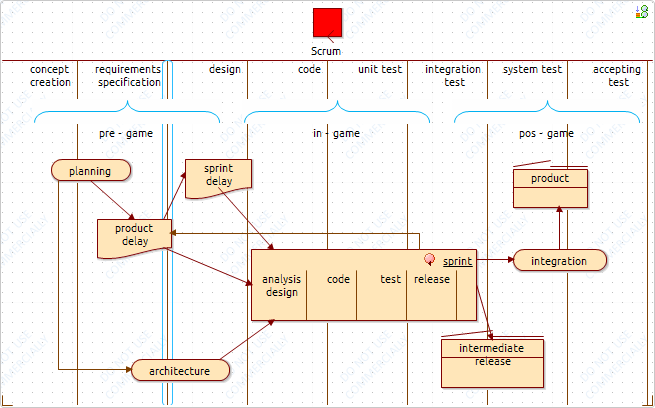
\includegraphics[width=0.7\linewidth]{proyecto/metodologia/imgs/Scrum}

%\lstinputlisting[language=java]{C:/a/Cliente.java}


\part{DISEÑO}
\chapter{Requerimientos}
\section{Introducción}
Como cualquier proyecto de cualquier indole, un punto fundamental, consiste en conocer cual es la necesidad o el problema que se desea resolver, lo cual conlleva a saber qué es lo que se debe realizar, para solventar tales necesidades. Esta es la idea básica de los requerimientos, definir cuales son los aspectos que se deben realizar para complacer las necesidades de un cliente.
\newpage

\section{Requerimientos del Cliente}
Se entienden como el qué es lo que el cliente esperará encontrar, cuando interactúe con la aplicación. Bajo la anterior premisa, se procede a definir los siguientes requerimientos de cliente:

\begin{enumerate}
	\item Mostrar todas las tareas pendientes.
	\item Mostrar las tareas pendientes por categoría.
	\item Mostrar las tareas pendientes por su tipo.
	\item Mostrar las tareas pendientes para una fecha.
	\item Mostrar las tareas pendientes por dificultad.
	\item Mostrar los horarios asignados para las tareas pendientes.
	\item Alertar de la próxima entrega de una tarea.
	\item Sugerir horarios de clase del usuario.
	\item Sugerir cuánto tiempo podría tomar una tarea.
	\item Sugerir tiempos de pausas activas durante la realización de una tarea.
	\item Advertir si se debe sacrificar algún espacio destinado a descanso.
	\item Advertir cuando no se alcanzará a terminar una tarea para una fecha especificada.
\end{enumerate}
\chapter{Interacción}
\section{Introducción}
cntenido...
\newpage
\chapter{Clases}
\section{Introducción}
cntenido...
\newpage
\chapter{Patrones}
\section{Introducción}
cntenido...
\newpage

\section{Prototipo}




\chapter{Estados}
\section{Introducción}
cntenido...
\newpage
\chapter{Componentes}
\section{Introducción}
cntenido...
\newpage
\chapter{Nodos}
\section{Introducción}
Un diagrama de nodos o de despliegue muestra las relaciones físicas de los nodos que la componen, además de cómo se reparten los nodos en cada nodo. Algunas de las ventajas de el uso de este tipo  de diagramas es la visión holística que se puede tener del proyecto, ya que muestra la relación y distribución de la parte de hardware y software. El problema de esto es que al ser tan general no se pueden vislumbrar algunos detalles que si se pueden ver en otro tipo de diagramas.
\section{Marco Teórico}
Un diagrama de despliegue se compone de:
\begin{itemize}
\item Nodo: Es un elemento de hardware o software que se muestra como una caja en tres dimensiones.
\begin{figure}[H]
	\centering
	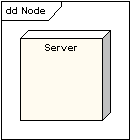
\includegraphics[width=1\linewidth]{diseno/nodos/imgs/1}
	\caption{Nodo. Imagen tomada de internet}
	\label{fig:gantt}
\end{figure}

\item Instancia de nodo: Una instancia se puede distinguir de un nodo por el hecho de que su nombre esta subrayado y tiene dos puntos antes del tipo de nodo base. 
\begin{figure}[H]
	\centering
	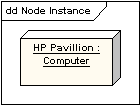
\includegraphics[width=1\linewidth]{diseno/nodos/imgs/2}
	\caption{Instancia de un nodo. Imagen tomada de internet}
	\label{fig:gantt}
\end{figure}

\item Estereotipo de nodo: Estereotipos estándar se proveen para los nodos, nombrados «cdrom», «cd-rom», «computer», «disk array», «pc», «pc client», «pc server», «secure», «server», «storage», «unix server», «user pc». Estos mostrarán un icono apropiado en la esquina derecha arriba del símbolo nodo.

\begin{figure}[H]
	\centering
	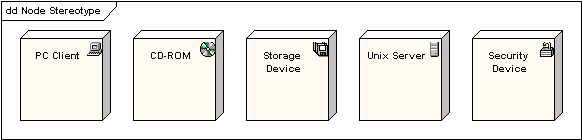
\includegraphics[width=1\linewidth]{diseno/nodos/imgs/3}
	\caption{Estereotipo de Nodo. Imagen tomada de internet}
	\label{fig:gantt}
\end{figure}

\item Artefacto: Un artefacto es un producto del proceso de desarrollo de software, que puede incluir los modelos del proceso como los casos de uso, los modelos de diseño, etc.

\begin{figure}[H]
	\centering
	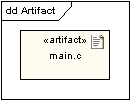
\includegraphics[width=1\linewidth]{diseno/nodos/imgs/4}
	\caption{Artefacto. Imagen tomada de internet}
	\label{fig:gantt}
\end{figure}

\end{itemize}

\section{Diagrama de nodos}

\chapter{Actividades}
\section{Introducción}
Los diagramas de actividades, junto a los de clases y casos de uso, son diagramas de comportamiento, ya que describen como funcionará ya sea de un algoritmo o incluso de un componente completo. Estos brindan grandes ventajas, como lo es mostrar un flujo de trabajo entre los usuarios y un sistema, clarificar ese tipo de procesos y traer simplificación.
Por ello, para describir cómo será el flujo de trabajo del software, se utilizarán los diagramas de actividades ya que estos permiten detallar en un lenguaje de alto nivel, los procesos que se llevan a cabo. 
\section{Marco Teórico}
Un diagrama de actividades está constituido por:
\begin{itemize}
\item Actividad: Es un comportamiento que describe una serie de acciones de forma determinada y organizada.
\begin{figure}[H]
	\centering
	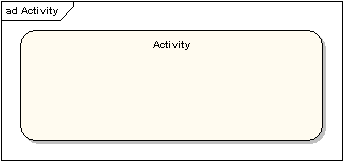
\includegraphics[width=0.5\linewidth]{diseno/actividades/imgs/1}
	\caption{Actividad. Imagen tomada de internet}
	\label{fig:gantt}
\end{figure}
\item Acción: Una acción representa un solo paso dentro de una actividad. Las acciones se denotan por rectángulos con las puntas redondeadas.
\begin{figure}[H]
	\centering
	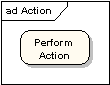
\includegraphics[width=0.5\linewidth]{diseno/actividades/imgs/3}
	\caption{Accion. Imagen tomada de internet}
	\label{fig:gantt}
\end{figure}
\item Flujo de control: Este muestra el flujo de una acción a otra. Se denota por una flecha.
\begin{figure}[H]
	\centering
	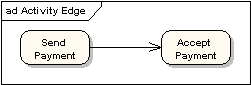
\includegraphics[width=0.5\linewidth]{diseno/actividades/imgs/2}
	\caption{Flujo de control. Imagen tomada de internet}
	\label{fig:gantt}
\end{figure}
\item Nodo inicial: Es el primer nodo, se describe por un gran punto negro.
\begin{figure}[H]
	\centering
	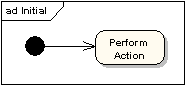
\includegraphics[width=0.5\linewidth]{diseno/actividades/imgs/6}
	\caption{Nodo inicial. Imagen tomada de internet}
	\label{fig:gantt}
\end{figure}
\item Nodo de decisión y combinación: Los nodos de decisión y combinación tienen la misma notación: una forma de diamante.  Los flujos de control que provienen de un nodo de decisión tendrán condiciones de guarda que permitirán el control para fluir si la condición de guarda se realiza.
\begin{figure}[H]
	\centering
	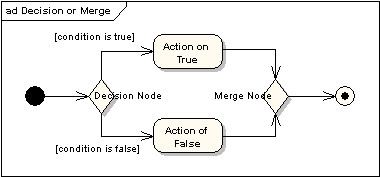
\includegraphics[width=0.5\linewidth]{diseno/actividades/imgs/4}
	\caption{Nodo de decisión y combinación. Imagen tomada de internet}
	\label{fig:gantt}
\end{figure}
\item Nodo de bifurcación y unión: Las bifurcaciones y uniones tienen la misma notación: una barra a la que llegan o de la que salen flujos de control). Estos indican el comienzo y final de hilos actuales de control.
\begin{figure}[H]
	\centering
	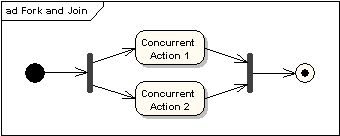
\includegraphics[width=0.5\linewidth]{diseno/actividades/imgs/5}
	\caption{Nodo de bifurcación y unión. Imagen tomada de internet}
	\label{fig:gantt}
\end{figure}
\item Particiones: 	Una partición se utiliza para separar acciones dentro de una actividad, se denota de la siguiente manera:
\begin{figure}[H]
	\centering
	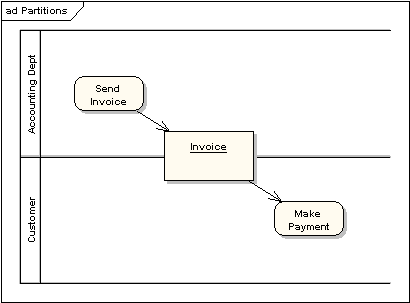
\includegraphics[width=0.5\linewidth]{diseno/actividades/imgs/7}
	\caption{Partición. Imagen tomada de internet}
	\label{fig:gantt}
\end{figure}
\end{itemize}
%http://www.sparxsystems.com.ar/resources/tutorial/uml2_activitydiagram.html
\section{Diagrama de actividades}
\part{REFLEXIONES}
k\chapter{Conclusiones}
\section{Introducción}
cntenido...
\newpage
%---bibliografia
\bibliographystyle{plain}
\bibliography{}

\end{document}